% appendix/rcuimpl/srcu.c

\section{Sleepable RCU Implementation}
\label{app:rcuimpl:Sleepable RCU Implementation}
\OriginallyPublished{Appendix}{app:rcuimpl:Sleepable RCU Implementation}{Sleepable RCU Implementation}{Linux Weekly News}{PaulEMcKenney2006c}

\begin{figure}[tb]
\centering
\resizebox{3in}{!}{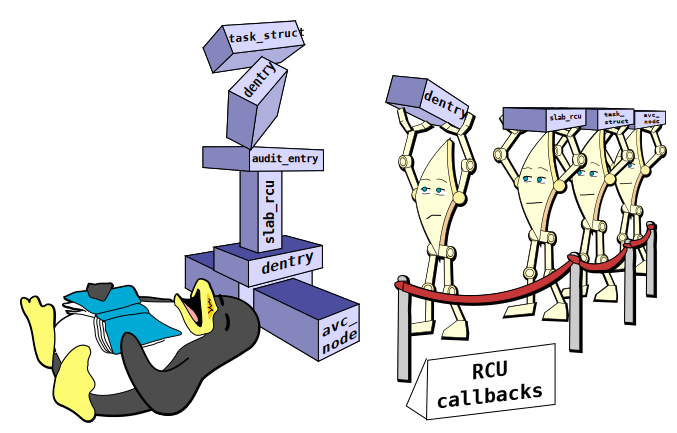
\includegraphics{cartoons/r-2014-RCU-callbacks}}
\caption{Sleeping While RCU Reading Considered Harmful}
\ContributedBy{Figure}{fig:app:rcuimpl:srcu:Sleeping While RCU Reading Considered Harmful}{Melissa Broussard}
\end{figure}

Classic RCU requires that read-side critical sections
obey the same rules
obeyed by the critical sections of pure spinlocks: blocking or sleeping
of any sort is strictly prohibited.
This has frequently been an obstacle to the use of RCU, and
Paul has received numerous requests for a ``sleepable RCU'' (SRCU) that
permits arbitrary sleeping (or blocking) within RCU read-side critical
sections.
Paul had previously rejected all such requests as unworkable, since arbitrary
sleeping in RCU read-side could indefinitely extend grace periods, which
in turn could result in arbitrarily large amounts of memory awaiting the
end of a grace period, which finally would result in disaster,
as fancifully depicted in
Figure~\ref{fig:app:rcuimpl:srcu:Sleeping While RCU Reading Considered Harmful},
with the most likely disaster being hangs due to memory exhaustion.
After all, any concurrency-control primitive that could result in
system hangs --- even when used correctly -- does not deserve to exist.

However, the realtime kernels that require spinlock critical sections
be preemptible~\cite{IngoMolnar05a} also require that RCU read-side critical
sections be preemptible~\cite{PaulMcKenney05b}.
Preemptible critical sections in turn require that lock-acquisition
primitives block in order to avoid deadlock,
which in turns means that both RCU's and spinlocks'
critical sections be able to block awaiting a lock.
However, these two forms of sleeping have the special property that
priority boosting and priority inheritance may be used to awaken
the sleeping tasks in short order.

Nevertheless,
use of RCU in realtime kernels was the first crack in the tablets
of stone on which were inscribed ``RCU read-side critical sections can never
sleep''.
That said, indefinite sleeping, such as blocking waiting for an
incoming TCP connection, is strictly verboten even in realtime kernels.

\QuickQuiz{}
	Why is sleeping prohibited within Classic RCU read-side
	critical sections?
\QuickQuizAnswer{
	Because sleeping implies a context switch, which in Classic RCU is
	a quiescent state, and RCU's grace-period detection requires that
	quiescent states never appear in RCU read-side critical sections.
} \QuickQuizEnd

\QuickQuiz{}
	Why not permit sleeping in Classic RCU read-side critical sections
	by eliminating context switch as a quiescent state, leaving user-mode
	execution and idle loop as the remaining quiescent states?
\QuickQuizAnswer{
	This would mean that a system undergoing heavy kernel-mode
	execution load (e.g., due to kernel threads) might never
	complete a grace period, which
	would cause it to exhaust memory sooner or later.
} \QuickQuizEnd

\subsection{SRCU Implementation Strategy}
\label{sec:app:rcuimpl:SRCU Implementation Strategy}

The primary challenge in designing an SRCU
is to prevent any given task sleeping in an RCU read-side
critical section from blocking an unbounded number of RCU callbacks.
SRCU uses two strategies to achieve this goal:
\begin{enumerate}
\item	refusing to provide asynchronous grace-period interfaces,
	such as the Classic RCU's \co{call_rcu()} API, and
\item	isolating grace-period detection within each subsystem using SRCU.
\end{enumerate}
The rationale for these strategies are discussed in the following sections.

\subsubsection{Abolish Asynchronous Grace-Period APIs}
\label{sec:app:rcuimpl:Abolish Asynchronous Grace-Period APIs}

The problem with the \co{call_rcu()} API is that a single thread can
generate an arbitrarily large number of blocks of memory awaiting a
grace period, as illustrated by the following:

\vspace{5pt}
\begin{minipage}[t]{\columnwidth}
\scriptsize
\begin{verbatim}
 1 while (p = kmalloc(sizeof(*p), GFP_ATOMIC))
 2   call_rcu(&p->rcu, f);
\end{verbatim}
\end{minipage}
\vspace{5pt}

In contrast, the analogous code using \co{synchronize_rcu()} can
have at most a single block of memory per thread awaiting a grace period:

\vspace{5pt}
\begin{minipage}[t]{\columnwidth}
\scriptsize
\begin{verbatim}
 1 while (p = kmalloc(sizeof(*p),
 2                    GFP_ATOMIC)) {
 3   synchronize_rcu();
 4   kfree(&p->rcu, f);
 5 }
\end{verbatim}
\end{minipage}
\vspace{5pt}

Therefore, SRCU provides an equivalent to \co{synchronize_rcu()}, but not
to \co{call_rcu()}.

\subsubsection{Isolate Grace-Period Detection}
\label{sec:app:rcuimpl:Isolate Grace-Period Detection}

In Classic RCU, a single read-side critical section could indefinitely
delay \emph{all} RCU callbacks, for example, as follows:

\vspace{5pt}
\begin{minipage}[t]{\columnwidth}
\scriptsize
\begin{verbatim}
 1 /* BUGGY: Do not use!! */
 2 rcu_read_lock();
 3 schedule_timeout_interruptible(longdelay);
 4 rcu_read_unlock();
\end{verbatim}
\end{minipage}
\vspace{5pt}

This sort of behavior might be tolerated if RCU were used only within
a single subsystem that was carefully designed to withstand long-term
delay of grace periods.
It is the fact that a single RCU read-side bug in one isolated subsystem can
delay \emph{all} users of RCU that forced these long-term RCU read-side
delays to be abolished.

One way around this issue is for grace-period detection to be performed
on a subsystem-by-subsystem basis, so that a lethargic RCU reader will
delay grace periods only within that reader's subsystem.
Since each subsystem can have only a bounded number of memory blocks
awaiting a grace period, and since the number of subsystems is also
presumably bounded, the total amount of memory awaiting a grace period
will also be bounded.
The designer of a given subsystem is responsible for: (1) ensuring that
SRCU read-side sleeping is bounded and (2) limiting the amount of memory
waiting for \co{synchronize_srcu()}.\footnote{
	For example, an SRCU-protected hash table might have a lock
	per hash chain, thus allowing at most one block per hash
	chain to be waiting for \co{synchronize_srcu()}.}

This is precisely the approach that SRCU takes, as described in the
following section.

\subsection{SRCU API and Usage}
\label{sec:app:rcuimpl:SRCU API and Usage}

The SRCU API is shown in Figure~\ref{fig:app:rcuimpl:SRCU API}.
The following sections describe how to use it.

\begin{figure}[htbp]
{ \scriptsize
\begin{verbatim}
int init_srcu_struct(struct srcu_struct *sp);
void cleanup_srcu_struct(struct srcu_struct *sp);
int srcu_read_lock(struct srcu_struct *sp);
void srcu_read_unlock(struct srcu_struct *sp, int idx);
void synchronize_srcu(struct srcu_struct *sp);
long srcu_batches_completed(struct srcu_struct *sp);
\end{verbatim}
}
\caption{SRCU API}
\label{fig:app:rcuimpl:SRCU API}
\end{figure}

\subsubsection{Initialization and Cleanup}
\label{sec:app:rcuimpl:Initialization and Cleanup}

Each subsystem using SRCU must create an
\co{struct} \co{srcu_struct},
either by declaring a variable of this type or by
dynamically allocating the memory, for example, via \co{kmalloc()}.
Once this structure is in place, it must be initialized via
\co{init_srcu_struct()}, which returns zero for success or an error
code for failure (for example, upon memory exhaustion).

If the \co{struct} \co{srcu_struct} is dynamically allocated, then
\co{cleanup_srcu_struct()} must be called before it is freed.
Similarly, if the \co{struct} \co{srcu_struct} is a variable declared within
a Linux kernel module, then \co{cleanup_srcu_struct()} must be called
before the module is unloaded.
Either way, the caller must take care to ensure that all SRCU read-side
critical sections have completed (and that no more will commence) before
calling \co{cleanup_srcu_struct()}.
One way to accomplish this is described in
Section~\ref{sec:app:rcuimpl:Cleaning Up Safely}.

\subsubsection{Read-Side Primitives}
\label{sec:app:rcuimpl:Read-Side Primitives}

The read-side \co{srcu_read_lock()} and \co{srcu_read_unlock()} primitives
are used as shown:

\vspace{5pt}
\begin{minipage}[t]{\columnwidth}
\scriptsize
\begin{verbatim}
 1 idx = srcu_read_lock(&ss);
 2 /* read-side critical section. */
 3 srcu_read_unlock(&ss, idx);
\end{verbatim}
\end{minipage}
\vspace{5pt}

The \co{ss} variable is the \co{struct} \co{srcu_struct} whose initialization
was described in Section~\ref{sec:app:rcuimpl:Initialization and Cleanup},
and the \co{idx} variable is an integer that in effect tells
\co{srcu_read_unlock()} the grace period during which the corresponding
\co{srcu_read_lock()} started.

This carrying of an index is a departure from the RCU API, which,
when required, stores the equivalent information in the task structure.
However, since a given task could potentially occupy an arbitrarily large
number of nested SRCU read-side critical sections, SRCU cannot
reasonably store this index in the task structure.

\subsubsection{Update-Side Primitives}
\label{sec:app:rcuimpl:Update-Side Primitives}

The \co{synchronize_srcu()} primitives may be used as shown below:

\vspace{5pt}
\begin{minipage}[t]{\columnwidth}
\scriptsize
\begin{verbatim}
 1 list_del_rcu(p);
 2 synchronize_srcu(&ss);
 3 kfree(p);
\end{verbatim}
\end{minipage}
\vspace{5pt}

As one might expect by analogy with Classic RCU, this primitive blocks
until until after the completion of all SRCU read-side critical sections
that started before the \co{synchronize_srcu()} started, as shown
in Table~\ref{tab:app:rcuimpl:SRCU Update and Read-Side Critical Sections}.
Here, CPU~1 need only wait for the completion of CPU~0's SRCU read-side
critical section.
It need not wait for the completion of CPU~2's SRCU read-side critical
section, because CPU~2 did not start this critical section until \emph{after}
CPU~1 began executing \co{synchronize_srcu()}.
Finally, CPU~1's \co{synchronize_srcu()} need not wait for CPU~3's
SRCU read-side critical section, because CPU~3 is using \co{s2} rather
than \co{s1} as its \co{struct} \co{srcu_struct}.
CPU~3's SRCU read-side critical section is thus related to a different
set of grace periods than those of CPUs~0 and 2.

\begin{table*}[htb]
\scriptsize
\centering
\begin{tabular}{r|l|l|l|l}
	& \multicolumn{1}{c|}{CPU 0} &
		\multicolumn{1}{c|}{CPU 1} &
			\multicolumn{1}{c|}{CPU 2} &
				\multicolumn{1}{c}{CPU 3} \\
	\hline
	\hline
	1 & \co{i0 = srcu_read_lock(&s1)} & & &
				\co{i3 = srcu_read_lock(&s2)} \\
	\hline
	2 &	& \co{synchronize_srcu(&s1)} enter & & \\
	\hline
	3 & 	&	& \co{i2 = srcu_read_lock(&s1)} & \\
	\hline
	4 & \co{srcu_read_unlock(&s1, i0)} & & & \\
	\hline
	5 &	& \co{synchronize_srcu(&s1)} exit & & \\
	\hline
	6 & 	&	 & \co{srcu_read_unlock(&s1, i2)} & \\
\end{tabular}
\caption{SRCU Update and Read-Side Critical Sections}
\label{tab:app:rcuimpl:SRCU Update and Read-Side Critical Sections}
\end{table*}

The \co{srcu_batches_completed()} primitive may be used to
monitor the progress of a given \co{struct} \co{srcu_struct}'s
grace periods.
This primitive is used in ``torture tests'' that validate SRCU's operation.

\subsubsection{Cleaning Up Safely}
\label{sec:app:rcuimpl:Cleaning Up Safely}

Cleaning up SRCU safely can be a challenge, but fortunately many
uses need not do so.
For example, uses in operating-system kernels that are initialized at
boot time need not be cleaned up.
However, uses within loadable modules must clean up if the corresponding
module is to be safely unloaded.

In some cases, such as the RCU torture module,
only a small known set of threads are using the
SRCU read-side primitives against a particular \co{struct} \co{srcu_struct}.
In these cases, the module-exit code need only kill that set of threads,
wait for them to exit, and then clean up.

In other cases, for example, for device drivers, any thread in the
system might be using the SRCU read-side primitives.
Although one could apply the method of the previous paragraph, this
ends up being equivalent to a full reboot, which can be unattractive.
Figure~\ref{fig:app:rcuimpl:SRCU Safe Cleanup} shows one way that cleanup
could be accomplished without a reboot.

\begin{figure}[htbp]
{ \scriptsize
\begin{verbatim}
  1 int readside(void)
  2 {
  3   int idx;
  4
  5   rcu_read_lock();
  6   if (nomoresrcu) {
  7     rcu_read_unlock();
  8     return -EINVAL;
  9   }
 10   idx = srcu_read_lock(&ss);
 11   rcu_read_unlock();
 12   /* SRCU read-side critical section. */
 13   srcu_read_unlock(&ss, idx);
 14   return 0;
 15 }
 16
 17 void cleanup(void)
 18 {
 19   nomoresrcu = 1;
 20   synchronize_rcu();
 21   synchronize_srcu(&ss);
 22   cleanup_srcu_struct(&ss);
 23 }
\end{verbatim}
}
\caption{SRCU Safe Cleanup}
\label{fig:app:rcuimpl:SRCU Safe Cleanup}
\end{figure}

The \co{readside()} function overlaps an RCU and an SRCU read-side
critical section, with the former running from lines~5-11 and the
latter running from lines 10-13.
The RCU read-side critical section uses Pure
%
% RCU\IfInBook{ (see Section~\ref{sec:advsync:Pure RCU})}
% 	    {~\cite{PaulEdwardMcKenneyPhD}}
%
RCU~\cite{PaulEdwardMcKenneyPhD}
%
to guard the
value of the \co{nomoresrcu} variable.
If this variable is set, we are cleaning up, and therefore must not enter
the SRCU read-side critical section, so we return \co{-EINVAL} instead.
On the other hand, if we are not yet cleaning up, we proceed into the
SRCU read-side critical section.

The \co{cleanup()} function first sets the \co{nomoresrcu} variable
on line~19, but then must wait for all currently executing RCU read-side
critical sections to complete via the \co{synchronize_rcu()} primitive
on line~20.
Once the \co{cleanup()} function reaches line~21, all calls to
\co{readside()} that could possibly have seen \co{nomorersrcu} equal
to zero must have already reached line~11, and therefore already must
have entered their SRCU read-side critical section.
All future calls to \co{readside()} will exit via line~8, and will thus
refrain from entering the read-side critical section.

Therefore, once \co{cleanup()} completes its call to
\co{synchronize_srcu()} on line~21, all SRCU read-side critical sections
will have completed, and no new ones will be able to start.
It is therefore safe on line~22 to call \co{cleanup_srcu_struct()}
to clean up.

\subsection{Implementation}
\label{sec:app:rcuimpl:Implementation}

This section describes SRCU's data structures, initialization and
cleanup primitives, read-side primitives, and update-side primitives.

\subsubsection{Data Structures}
\label{sec:app:rcuimpl:Data Structures}

SRCU's data structures are shown in
Figure~\ref{fig:app:rcuimpl:SRCU Data Structures},
and are depicted schematically in
Figure~\ref{fig:app:whymb:SRCU Data-Structure Diagram}.
The \co{completed} field is a count of the number of grace periods
since the \co{struct} \co{srcu} was initialized, and as shown in the
diagram, its low-order bit is used to index the
\co{struct} \co{srcu_struct_array}.
The \co{per_cpu_ref} field points to the array, and the
\co{mutex} field is used to permit but one \co{synchronize_srcu()} at
a time to proceed.

\begin{figure}[htbp]
{ \scriptsize
\begin{verbatim}
 1 struct srcu_struct_array {
 2   int c[2];
 3 };
 4 struct srcu_struct {
 5   int completed;
 6   struct srcu_struct_array *per_cpu_ref;
 7   struct mutex mutex;
 8 };
\end{verbatim}
}
\caption{SRCU Data Structures}
\label{fig:app:rcuimpl:SRCU Data Structures}
\end{figure}

\begin{figure}[htb]
\centering
% \resizebox{3in}{!}{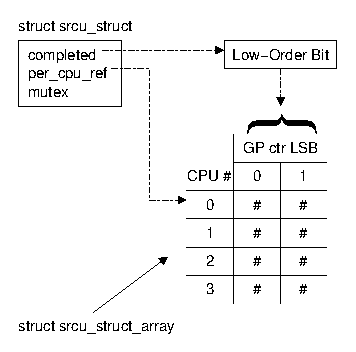
\includegraphics{appendix/rcuimpl/srcuds}}
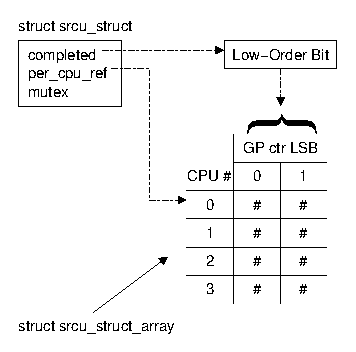
\includegraphics{appendix/rcuimpl/srcuds}
\caption{SRCU Data-Structure Diagram}
\label{fig:app:whymb:SRCU Data-Structure Diagram}
\end{figure}

\subsubsection{Initialization Implementation}
\label{sec:app:rcuimpl:Initialization Implementation}

SRCU's initialization function, \co{init_srcu_struct()}, is shown in
Figure~\ref{fig:app:rcuimpl:SRCU Initialization}.
This function simply initializes the fields in the
\co{struct} \co{srcu_struct}, returning zero if initialization succeeds
or \co{-ENOMEM} otherwise.

\begin{figure}[htbp]
{ \scriptsize
\begin{verbatim}
  1 int init_srcu_struct(struct srcu_struct *sp)
  2 {
  3   sp->completed = 0;
  4   mutex_init(&sp->mutex);
  5   sp->per_cpu_ref =
  6     alloc_percpu(struct srcu_struct_array);
  7   return (sp->per_cpu_ref ? 0 : -ENOMEM);
  8 }
\end{verbatim}
}
\caption{SRCU Initialization}
\label{fig:app:rcuimpl:SRCU Initialization}
\end{figure}

SRCU's cleanup functions are shown in
Figure~\ref{fig:app:rcuimpl:SRCU Cleanup}.
The main cleanup function, \co{cleanup_srcu_struct()} is shown
on lines~19-29 of this figure, however, it immediately invokes
\co{srcu_readers_active()}, shown on lines~13-17 of this figure,
to verify that there are no readers currently using this
\co{struct} \co{srcu_struct}.

The \co{srcu_readers_active()} function simply returns the sum of
\co{srcu_readers_active_idx()} on both possible indexes,
while \co{srcu_readers_active_idx()}, as shown on lines~1-11,
sums up the per-CPU counters corresponding to the specified index,
returning the result.

If the value returned from \co{srcu_readers_active()} is non-zero,
then \co{cleanup_srcu_struct()} issues a warning on line~24 and
simply returns on lines~25 and 26, declining to destroy a
\co{struct} \co{srcu_struct} that is still in use.
Such a warning always indicates a bug, and given that the bug
has been reported, it is better to allow the system to continue
with a modest memory leak than to introduce possible memory corruption.

Otherwise, \co{cleanup_srcu_struct()} frees the array of per-CPU
counters and \co{NULL}s the pointer on lines~27 and 28.

\begin{figure}[htbp]
{ \scriptsize
\begin{verbatim}
  1 int srcu_readers_active_idx(struct srcu_struct *sp,
  2                             int idx)
  3 {
  4   int cpu;
  5   int sum;
  6
  7   sum = 0;
  8   for_each_possible_cpu(cpu)
  9     sum += per_cpu_ptr(sp->per_cpu_ref, cpu)->c[idx];
 10   return sum;
 11 }
 12
 13 int srcu_readers_active(struct srcu_struct *sp)
 14 {
 15   return srcu_readers_active_idx(sp, 0) +
 16          srcu_readers_active_idx(sp, 1);
 17 }
 18
 19 void cleanup_srcu_struct(struct srcu_struct *sp)
 20 {
 21   int sum;
 22
 23   sum = srcu_readers_active(sp);
 24   WARN_ON(sum);
 25   if (sum != 0)
 26     return;
 27   free_percpu(sp->per_cpu_ref);
 28   sp->per_cpu_ref = NULL;
 29 }
\end{verbatim}
}
\caption{SRCU Cleanup}
\label{fig:app:rcuimpl:SRCU Cleanup}
\end{figure}

\subsubsection{Read-Side Implementation}
\label{sec:app:rcuimpl:Read-Side Implementation}

The code implementing \co{srcu_read_lock()} is shown in
Figure~\ref{fig:app:rcuimpl:Read-Side Acquisition}.
This function has been carefully constructed to avoid the
need for memory barriers and atomic instructions.

Lines~5 and 11 disable and re-enable preemption, in order to force
the sequence of code to execute unpreempted on a single CPU.
Line~6 picks up the bottom bit of the grace-period counter, which will
be used to select which rank of per-CPU counters is to be used for this
SRCU read-side critical section.
The \co{barrier()} call on line~7 is a directive to the compiler
that ensures that the index is
fetched but once,\footnote{
	Please note that, despite the name, \co{barrier()}
	has absolutely no effect on the CPU's ability to
	reorder execution of both code and of memory accesses.}
so that the index used on line~9 is the same
one returned on line~12.
Lines~8-9 increment the selected counter for the current CPU.\footnote{
	It is important to note that the \co{smp_processor_id()} primitive
	has long-term meaning only if preemption is disabled.
	In absence of preemption disabling, a potential preemption
	immediately following execution of this primitive could
	cause the subsequent code to execute on some other CPU.}
Line~10 forces subsequent execution to occur \emph{after}
lines~8-9, in order to prevent to misordering of any code
in a non-\co{CONFIG_PREEMPT} build, but only
from the perspective of an intervening interrupt handler.
However, in a \co{CONFIG_PREEMPT} kernel, the required \co{barrier()}
call is embedded in the \co{preempt_enable()} on line~11, so the
\co{srcu_barrier()} is a no-op in that case.
Finally, line~12 returns the index so that it may be passed in to the
corresponding \co{srcu_read_unlock()}.

\begin{figure}[htbp]
{ \scriptsize
\begin{verbatim}
  1 int srcu_read_lock(struct srcu_struct *sp)
  2 {
  3   int idx;
  4
  5   preempt_disable();
  6   idx = sp->completed & 0x1;
  7   barrier();
  8   per_cpu_ptr(sp->per_cpu_ref,
  9               smp_processor_id())->c[idx]++;
 10   srcu_barrier();
 11   preempt_enable();
 12   return idx;
 13 }
\end{verbatim}
}
\caption{SRCU Read-Side Acquisition}
\label{fig:app:rcuimpl:Read-Side Acquisition}
\end{figure}

The code for \co{srcu_read_unlock()} is shown in
Figure~\ref{fig:app:rcuimpl:Read-Side Release}.
Again, lines~3 and 7 disable and re-enable preemption so that the
whole code sequence executes unpreempted on a single CPU.
In \co{CONFIG_PREEMPT} kernels, the \co{preempt_disable()} on line~3
contains a \co{barrier()} primitive, otherwise, the \co{barrier()}
is supplied by line~4.
Again, this directive forces the subsequent code to execute after
the critical section from the perspective of intervening
interrupt handlers.
Lines~5 and 6 decrement the counter for this CPU, but with the same
index as was used by the corresponding \co{srcu_read_lock()}.

\begin{figure}[htbp]
{ \scriptsize
\begin{verbatim}
  1 void srcu_read_unlock(struct srcu_struct *sp, int idx)
  2 {
  3   preempt_disable();
  4   srcu_barrier();
  5   per_cpu_ptr(sp->per_cpu_ref,
  6               smp_processor_id())->c[idx]--;
  7   preempt_enable();
  8 }
\end{verbatim}
}
\caption{SRCU Read-Side Release}
\label{fig:app:rcuimpl:Read-Side Release}
\end{figure}

The key point is that a given CPU's counters
can be observed by other CPUs only in
cooperation with that CPU's interrupt handlers.
These interrupt handlers are responsible for ensuring that any needed
memory barriers are executed prior to observing the counters.

\subsubsection{Update-Side Implementation}
\label{sec:app:rcuimpl:Update-Side Implementation}

The key point behind SRCU is that \co{synchronize_sched()}
blocks until all currently-executing preempt-disabled regions of
code complete.
The \co{synchronize_srcu()} primitive makes heavy use of this effect,
as can be seen in
Figure~\ref{fig:app:rcuimpl:Update-Side Implementation}.

Line~5 takes a snapshot of the grace-period counter.
Line~6 acquires the mutex, and lines~7-10 check to see whether
at least two grace periods have elapsed since the snapshot,
and, if so, releases the lock and returns --- in this case, someone
else has done our work for us.
Otherwise, line~11 guarantees that any other CPU that sees the
incremented value of the grace period counter in \co{srcu_read_lock()}
also sees any changes made by this CPU prior to entering
\co{synchronize_srcu()}.
This guarantee is required to make sure that any SRCU read-side
critical sections not blocking the next grace period have seen
any prior changes.

Line~12 fetches the bottom bit of the grace-period counter for later
use as an index into the per-CPU counter arrays, and then line~13
increments the grace-period counter.
Line~14 then waits for any currently-executing \co{srcu_read_lock()}
to complete, so that by the time that we reach line~15, all
extant instances of \co{srcu_read_lock()} will be using the updated
value from \co{sp->completed}.
Therefore, the counters sampled in by \co{srcu_readers_active_idx()}
on line~15 are guaranteed to
be monotonically decreasing, so that once their sum reaches zero, it
is guaranteed to stay there.

However, there are no memory barriers in the \co{srcu_read_unlock()}
primitive, so the CPU is within its rights to reorder the counter
decrement up into the SRCU critical section, so that references to
an SRCU-protected data structure could in effect ``bleed out'' of the
SRCU critical section.
This scenario is addressed by the \co{synchronize_sched()} on line~17,
which blocks until all other CPUs executing in \co{preempt_disable()}
code sequences (such as that in \co{srcu_read_unlock()}) complete these
sequences.
Because completion of a given \co{preempt_disable()} code sequence
is observed from the CPU executing that sequence, completion of the
sequence implies completion of any prior SRCU read-side critical section.
Any required memory barriers are supplied by the code making the
observation.

At this point, it is therefore safe to release the mutex as shown
on line~18 and return to the caller, who can now be assured that
all SRCU read-side critical sections sharing the same
\co{struct} \co{srcu_struct}
will observe any update made prior to the call to \co{synchronize_srcu()}.

\begin{figure}[htbp]
{ \scriptsize
\begin{verbatim}
  1 void synchronize_srcu(struct srcu_struct *sp)
  2 {
  3   int idx;
  4
  5   idx = sp->completed;
  6   mutex_lock(&sp->mutex);
  7   if ((sp->completed - idx) >= 2) {
  8     mutex_unlock(&sp->mutex);
  9     return;
 10   }
 11   synchronize_sched();
 12   idx = sp->completed & 0x1;
 13   sp->completed++;
 14   synchronize_sched();
 15   while (srcu_readers_active_idx(sp, idx))
 16     schedule_timeout_interruptible(1);
 17   synchronize_sched();
 18   mutex_unlock(&sp->mutex);
 19 }
\end{verbatim}
}
\caption{SRCU Update-Side Implementation}
\label{fig:app:rcuimpl:Update-Side Implementation}
\end{figure}

\QuickQuiz{}
	Why is it OK to assume that updates separated by
	\co{synchronize_sched()} will be performed in order?
\QuickQuizAnswer{
	Because this property is required for the \co{synchronize_sched()}
	aspect of RCU to work at all.
	For example, consider a code sequence that removes an object
	from a list, invokes \co{synchronize_sched()}, then frees
	the object.
	If this property did not hold, then that object might appear
	to be freed before it was
	removed from the list, which is precisely the situation that
	\co{synchronize_sched()} is supposed to prevent!
} \QuickQuizEnd

\QuickQuiz{}
	Why must line~17 in \co{synchronize_srcu()}
	(Figure~\ref{fig:app:rcuimpl:Update-Side Implementation})
	precede the release of the mutex on line~18?
	What would have to change to permit these two lines to be
	interchanged?
	Would such a change be worthwhile?
	Why or why not?
\QuickQuizAnswer{
	Suppose that the order was reversed, and that CPU~0
	has just reached line~13 of
	\co{synchronize_srcu()}, while both CPU~1 and CPU~2 start executing
	another \co{synchronize_srcu()} each, and CPU~3 starts executing a
	\co{srcu_read_lock()}.
	Suppose that CPU~1 reaches line~6 of \co{synchronize_srcu()}
	just before CPU~0 increments the counter on line~13.
	Most importantly, suppose that
	CPU~3 executes \co{srcu_read_lock()}
	out of order with the following SRCU read-side critical section,
	so that it acquires a reference to some SRCU-protected data
	structure \emph{before} CPU~0 increments \co{sp->completed}, but
	executes the \co{srcu_read_lock()} \emph{after} CPU~0 does
	this increment.
	
	Then CPU~0 will \emph{not} wait for CPU~3 to complete its
	SRCU read-side critical section before exiting the ``while''
	loop on lines~15-16 and releasing the mutex (remember, the
	CPU could be reordering the code).
	
	Now suppose that CPU~2 acquires the mutex next,
	and again increments \co{sp->completed}.
	This CPU will then have to wait for CPU~3 to exit its SRCU
	read-side critical section before exiting the loop on
	lines~15-16 and releasing the mutex.
	But suppose that CPU~3 again executes out of order,
	completing the \co{srcu_read_unlock()} prior to
	executing a final reference to the pointer it obtained
	when entering the SRCU read-side critical section.

	CPU~1 will then acquire the mutex, but see that the
	\co{sp->completed} counter has incremented twice, and
	therefore take the early exit.
	The caller might well free up the element that CPU~3 is
	still referencing (due to CPU~3's out-of-order execution).

	To prevent this perhaps improbable, but entirely possible,
	scenario, the final \co{synchronize_sched()} must precede
	the mutex release in \co{synchronize_srcu()}.

	Another approach would be to change to comparison on
	line~7 of \co{synchronize_srcu()} to check for at
	least three increments of the counter.
	However, such a change would increase the latency of a
	``bulk update'' scenario, where a hash table is being updated
	or unloaded using multiple threads.
	In the current code, the latency of the resulting concurrent
	\co{synchronize_srcu()} calls would take at most two SRCU
	grace periods, while with this change, three would be required.

	More experience will be required to determine which approach
	is really better.
	For one thing, there must first be some use of SRCU with
	multiple concurrent updaters.
} \QuickQuizEnd

\subsection{SRCU Summary}
\label{sec:app:rcuimpl:SRCU Summary}

SRCU provides an RCU-like set of primitives that permit general
sleeping in the SRCU read-side critical sections.
However, it is important to note that SRCU has been used only in
prototype code, though it has passed the RCU torture test.
It will be very interesting to see what use, if any, SRCU sees
in the future.
